\section{碰 (40pts)}
瓦雷莎正在锻炼她的碰撞本领,她会去尝试冲撞一个静止的巨石。下面让我们来帮她分析一下情况,我们将他们抽象为两个质点,分别为\(m_1\)和\(m_2\),其中\(m_1\)为瓦雷莎,\(m_2\)为静止的巨石。瓦雷莎以初始动量\(p_0\)向右冲撞巨石,考虑相对论效应,已知光速为\(c\),则瓦雷莎初始能量为\(E_1 = \sqrt{p_0^2c^2 + m_1^2c^4}\)。如图\ref{peng1} 所示:
\begin{figure}[htbp]
	\centering
	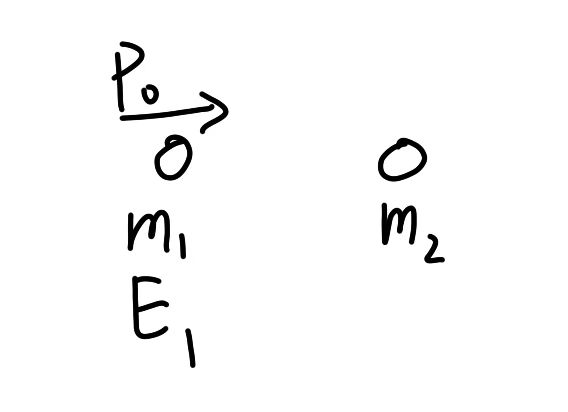
\includegraphics[width=0.3\textwidth]{peng1}
	\caption{碰撞示意图.}
	\label{peng1}
\end{figure}
\begin{enumerate}
	\item 我们先为这个分析打一个基础:已知空间中有\(n\)个质点,它们的动量分别为\(\vec{p}_1,\vec{p}_2,\cdots,\vec{p}_n\),能量分别为\(E_1,E_2,\cdots,E_n\),请你证明:存在一个参考系,它相对于当前参考系的速度为\(\vec{\beta}_c c\), 使得在这个参考系中,所有的质点的总动量为0,并求出\(\vec{\beta}_c\)的表达式。(12pts)
	\item 现在回来分析瓦雷莎的情况,请问什么情况下她会直接被巨石原路反弹?请给出条件,当不会反弹时,求出她的最大可能的偏离原来方向的角度。(28pts)
\end{enumerate}